\documentclass[aspectratio=169]{beamer}
% \documentclass[aspectratio=169]{beamer} % proyector 16:9 | Ref:  https://en.wikibooks.org/wiki/LaTeX/Presentations
\usetheme{Boadilla}
\beamertemplatenavigationsymbolsempty %% Sin barra navegación
\usecolortheme{beaver}


%% Spanska!
\usepackage[utf8]{inputenc}
\usepackage{lmodern} % no producia letras en matemático | Ref: https://tex.stackexchange.com/questions/250413/error-when-using-greek-symbol-in-subscript-in-beamer-presentation 
\usepackage[spanish]{babel}
\def\spanishoptions{argentina}

%% inclusión de gráficas
\usepackage{graphicx}	% instalar ghostscript-x para que el dvi muestre los eps
\graphicspath{ {./graphs/} {../figuras/} {../unlam_mep2023/graphs/}}
\usepackage{rotating}	% epígrafe rotado


\begin{document}

\title[A code centred mechanics subject]{A rational mechanics course where everything\\is made with Python code}
% \subtitle{Capitalizando lo desarrollado durante el confinamiento}
\author[vbettachini@unlam.edu.ar]{Bettachini, Víctor A.; Real, Mariano A.; Palazzo, Edgardo}
%\institute[]{
%	Ingeniería Mecánica, DIIT, UNLaM
%}
\date[2023-11-23]{
	New Media Pedagogy 23
}

\usebackgroundtemplate{
  
\includegraphics[width=\paperwidth, height=\paperheight]{diit_titre_background}
}	% unset background % https://tex.stackexchange.com/questions/201013/how-to-include-a-background-image-to-only-one-page-of-a-beamer-presentation

\begin{frame} 
  \titlepage
\end{frame}

\usebackgroundtemplate{
  
\includegraphics[width=\paperwidth, height=\paperheight]{diit_background}
} %% https://mprnotes.wordpress.com/2009/08/14/changing-background-image-of-latex-beamer/


\begin{frame}
	\frametitle{Value students and professors time}
	Licklider (1957): 85\% of ``thinking'' are actually mundane task (calculations, drawing, etc.)
	\pause
	\begin{block}{}
	  \begin{columns}[b]
			\begin{column}{0.25\textwidth}
				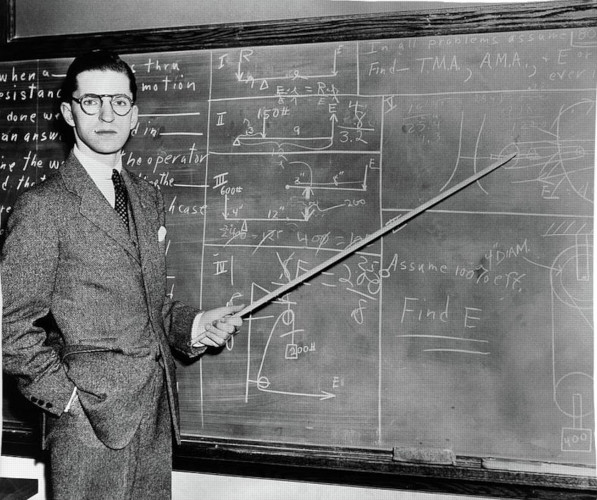
\includegraphics[width= \columnwidth]{1930s-1940s-man-teacher-professor-vintage-images}
			\end{column}
			\begin{column}{0.65\textwidth}
				Classroom and practice: an excercise on transcription
				\begin{itemize}[<+->]
					\item Professor: lessons \(\xrightarrow{by\, heart}\) blackboard/slides
					\item Student: blackboard/slides \(\xrightarrow{copies}\) notebooks
					\item Práctice \textbf{reiterate} diagrames, calculations, etc.
					\item Boredom \(\implies \downarrow\) concentration on the subject
				\end{itemize}
			\end{column}
		\end{columns}
	\end{block}
	\pause
	\begin{block}{}
	  \begin{columns}[b]
			\begin{column}{0.25\textwidth}
				\includegraphics[width= \columnwidth]{"Screenshot 2023-09-18 at 12-24-03 Google Colaboratory"}
			\end{column}
			\begin{column}{0.65\textwidth}
				\begin{itemize}[<+->]
					\item Professor: ideas \(\rightarrow\) new code/notes in repository
					\item Student: course repository \(\rightarrow\) its own modifiable one
					\item Use code to solve problems = \textbf{recycle} professor's code
					\item Modifiying it solves different problems
				\end{itemize}
			\end{column}
		\end{columns}
	\end{block}
\end{frame}


\begin{frame}
	\frametitle{Engineering students must take advantage of code at every single lecture}
	\pause
	\begin{block}{}
		\begin{itemize}[<+->]
			\item Currently they use a pocket calculator \textbf{after they learnt} learning arithmetics at school
			\item They'll employ computational algebra \textbf{after they learnt} algebra and calculus
			\begin{itemize}[<+->]
				\item Focus on new skills, not in automatable calculations
				%\item Álgebra y análisis simbólico
				\item Employing numerical calculus they solve what is impossible in a blackboard/paper
			\end{itemize}
			\end{itemize}
		% \uncover<4->{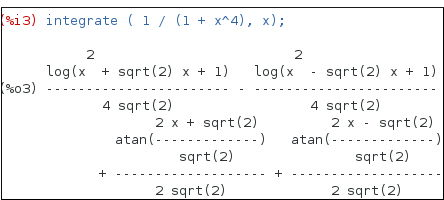
\includegraphics[height= 2cm]{ucarecdn}}
	\only<2>{\includegraphics[height= 2cm]{reglacalculadora}}
	\uncover<3->{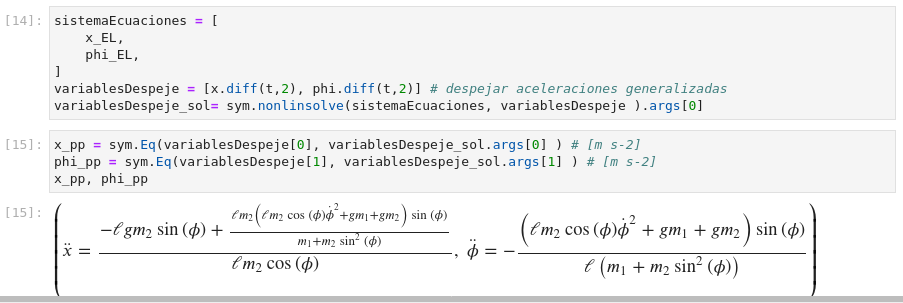
\includegraphics[width= 0.49\textwidth]{hard}}
	\uncover<5->{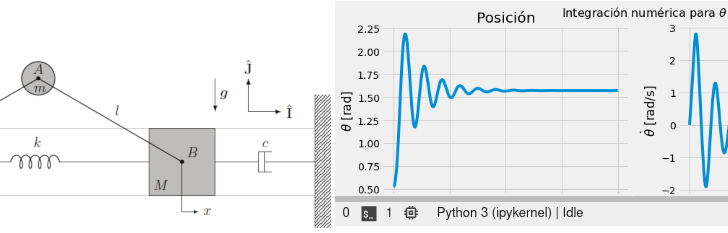
\includegraphics[width= 0.49\textwidth]{impracticable}}
	\end{block}
	\pause
	\begin{block}{}
		Papert (1980) ``...the best learning takes place when the learner takes charge''
		\begin{itemize}[<+->]
			\item An expample problem is solved by the professor provided code
			\item The student modifies it to solve other related problems
			\item Gradually he becomes autonomous by reusing not the provided but his own code
		\end{itemize}
	\end{block}
\end{frame}


\begin{frame}
	\frametitle{All course material can be edited on-line}
	\pause
	\begin{block}{On-line programmable notebook: text + equations + code}
		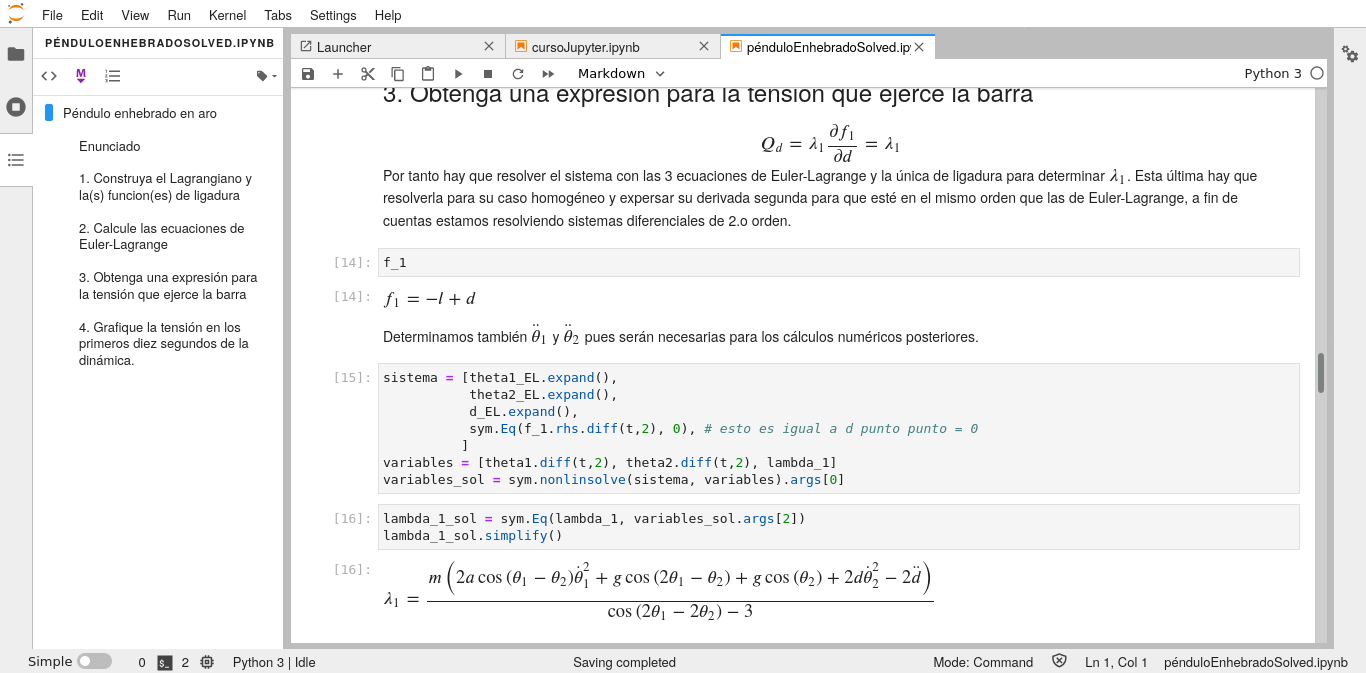
\includegraphics[width= \columnwidth]{screenshot_JupyterLab}
	\end{block}
\end{frame}


\begin{frame}
	\frametitle{Synchronical and asynchronical work on the code}
	\begin{block}{New theory alongisde its worked examples in programmable notebooks}
		\begin{itemize}[<+->]
			\item On-line 24/7 \textbf{asynchronical} consultations that are \textbf{public} for others to see
			\item \textbf{Remote collaboration} on multi-user notebooks
			\item Weekly meetings to \textbf{synchronically} unfinished assignments with TA's assistance
			\item On a weekly basis these \textbf{must} be turned-in for scoring
		\end{itemize}
	\end{block}
	\begin{columns}[b]<1->
    \begin{column}{0.35\textwidth}
			\begin{block}{Inverted classroom}
				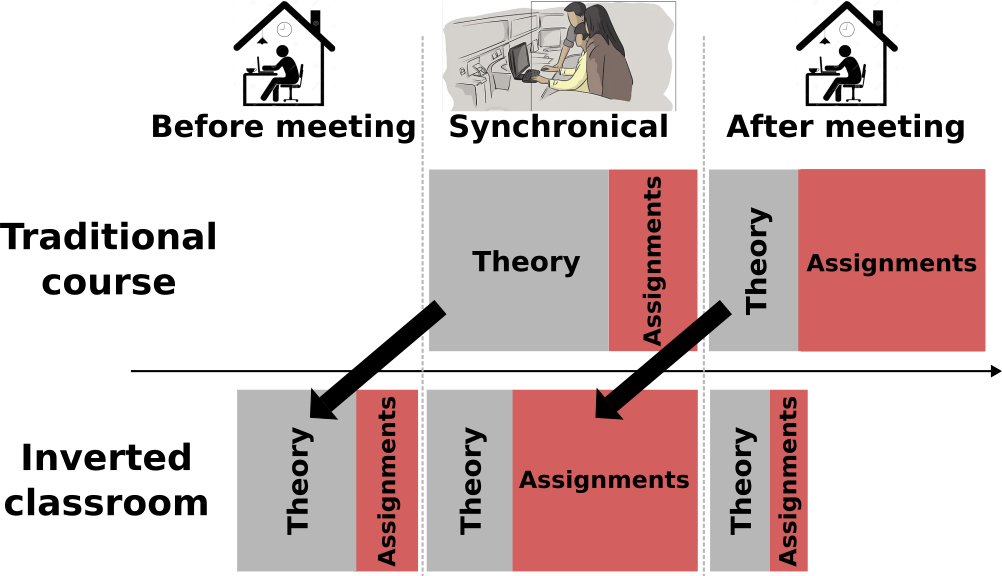
\includegraphics[width= \columnwidth]{invertedClassroomSchedule.png}
			\end{block}
    \end{column}
    \begin{column}{0.6\textwidth}
			\begin{block}{}
				\begin{tabular}{lll}
					\hline
					Synchronical & Theory & Assignments\\
					\hline
					Before & Read and apply  & Start them\\
					During & Consultations & Complete them\\
					% Durante & Aclarar dudas & \begin{tabular}{@{}c@{}}Terminarles\\(semanal)\end{tabular}\\
					After & \begin{tabular}{@{}l@{}}Additional\\consultations\end{tabular} & \begin{tabular}{@{}l@{}}TA's corrections\end{tabular}\\
					\hline
				\end{tabular}
			\end{block}
    \end{column}
  \end{columns}
\end{frame}



\begin{frame}
	\frametitle{Asynchronical corrections and remote assistance}
	\begin{block}{Student's work can be commented and edited in Google Colaboratory}
		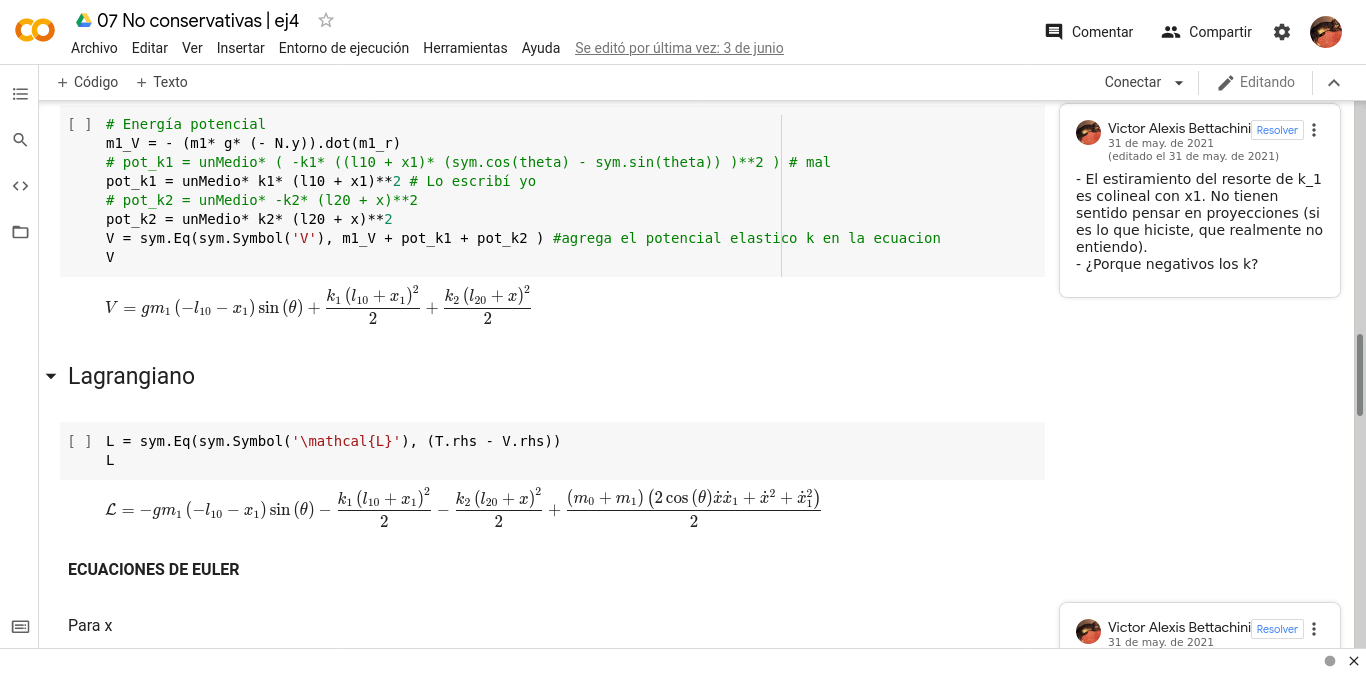
\includegraphics[width= \columnwidth]{comentariosColab}
	\end{block}
\end{frame}


\begin{frame}
	\frametitle{Individualized student follow-up at Microsoft Teams}
	\begin{block}{A record of the weekly turn-up of assignments}
		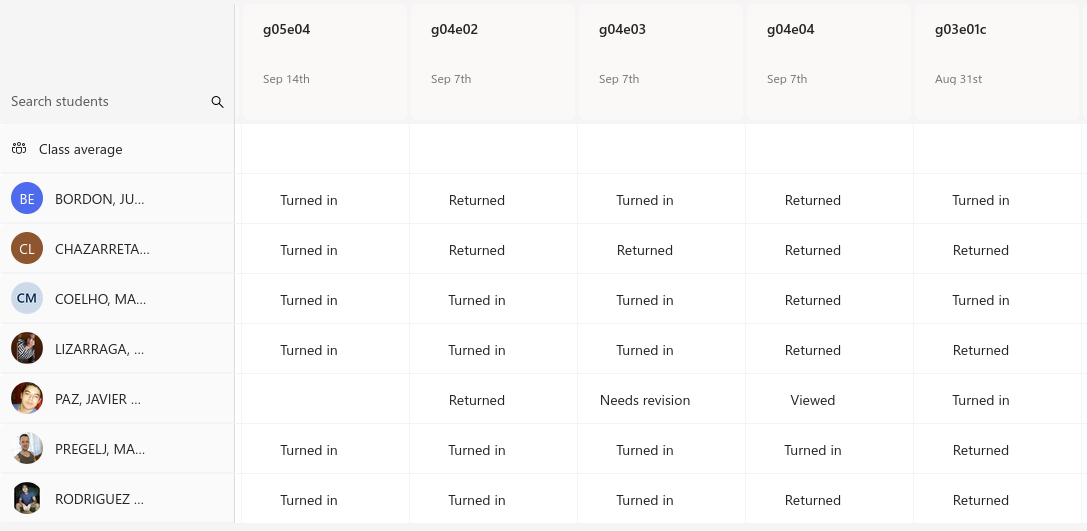
\includegraphics[width= \columnwidth]{seguimiento}
	\end{block}
\end{frame}


\begin{frame}
	\frametitle{Summary}
	\begin{block}{A course centred on code}
		\begin{itemize}[<+->]
			\item Theory: text + equations + executable cod in digital notebooks.
			\item Reinforced by: suggested bibliography and short professor's videos.
			\item assignments: professor's code recycling.
			\item On-line:
			\begin{itemize}[<+->]
				\item Remote collaboration and correction
				\item Doesn't require powerful nor at campus computers
				\item A dated record of each student's work
			\end{itemize}
		\end{itemize}
	\end{block}
	\begin{block}{Inverted classroom}
		\begin{itemize}[<+->]
			\item Theory: emphasis on student's autonomus reading
			\item Consultations: mostly on-line asynchronical and of public access
			\item TA personal assisantace when completing assignments in synchronical meetings
			%\item Práctica: Docente asiste personalmente cuando más se lo requiere, para finalizar ejercicios.
		\end{itemize}
	\end{block}
\end{frame}
	


\begin{frame}
	\frametitle{Current developments}
	\pause
	\begin{block}{}
		\begin{description}[<+->]
			\item [2023] Students feedback improved:
				\begin{itemize}
					\item Theory notes and code at repository
					\item Grading of assignments methodology\\
							Evaluating each one of them \(\rightarrow\) higher student's performance
				\end{itemize}
			\item [2024] 
				\begin{itemize}
					\item A course on optics and waves will incorporate part of the methodology
					\item AI assistance in code generation employing \emph{GitHub Copilot}
				\end{itemize}
			% \item [202x] Difundir la metodología en el DIIT.
		\end{description}
	\end{block}
	\uncover<6->{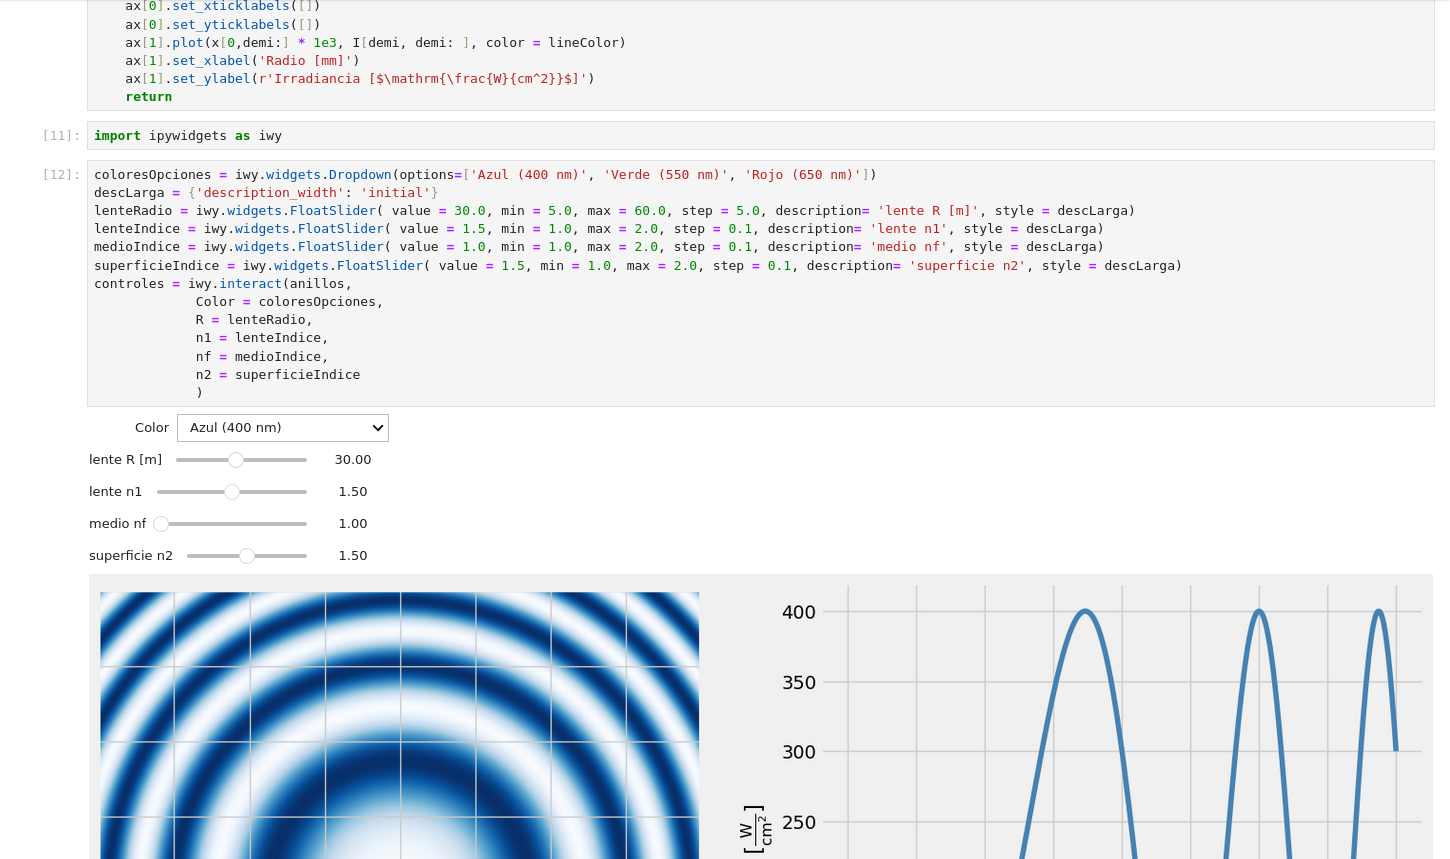
\includegraphics[height= 3cm]{cuñaAnillosN}}
	\uncover<7->{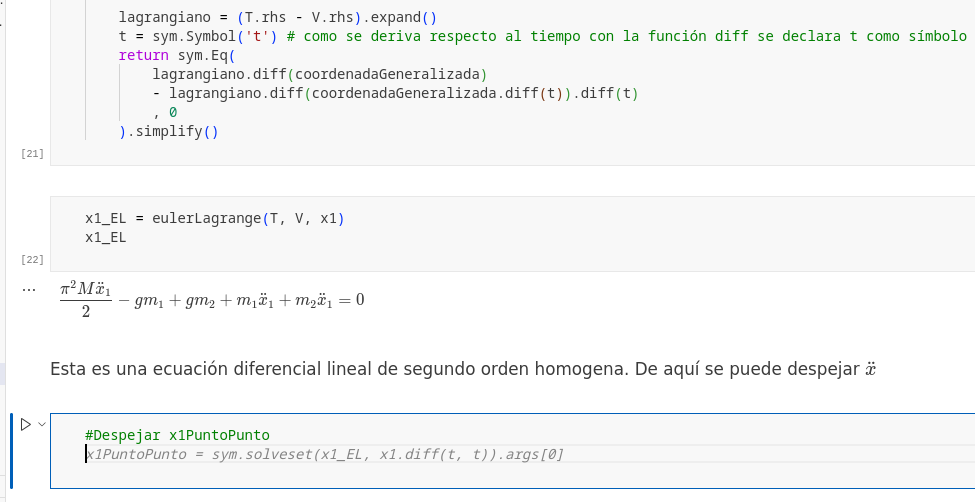
\includegraphics[height= 3cm]{copilot}}
\end{frame}


\end{document}
